%%%%%%%%%%%%%%%%%%%%%%%%%%%%%%%%%%%%%%%%%%%%%%%%%%%%%%%%%%%%%%%%%%%%%%%
\documentclass
  [ 11pt
  %twoside            % beidseitiger Druck
  , openright          % Kapitel beginnen auf einer rechten Seite
  , listof=totoc       % Verzeichnisse im Inhaltsverzeichnis
  , bibliography=totoc % Literaturverzeichnis im Inhaltsverzeichnis
  , parskip=full       % Absätze durch einen vergrößerten Zeilenabstand getrennt
%  , draft              % Entwurfsversion
  ]{scrreprt}          % Dokumentenklasse: KOMA-Script Buch

\input{stuff/header}

\begin{document}

%%%%%%%%%%%%%%%%%%%%%%%%%%%%%%%%%%%%%%%%%%%%%%%%%%%%%%%%%%%%%%%%%%%

% Titelseite
\newgeometry{left=3cm,right=2cm,top=2.0cm,bottom=2.0cm}
\include{stuff/titelseite}
\restoregeometry

%%%%%%%%%%%%%%%%%%%%%%%%%%%%%%%%%%%%%%%%%%%%%%%%%%%%%%%%%%%%%%%%%%%

% Mehr Platz für Nummerierung benötigt in Verzeichnissen, wenn ein Kapitel 10 oder mehr Bilder hat
\DeclareTOCStyleEntry[numwidth=3em]{tocline}{figure} % Für Abbildungsverzeichnis
%\DeclareTOCStyleEntry[numwidth=3em]{tocline}{table} % Für Tabellenverzeichnis

\pagenumbering{Roman}

\tableofcontents
\listoffigures
\listoftables
\cleardoublepage

%%%%%%%%%%%%%%%%%%%%%%%%%%%%%%%%%%%%%%%%%%%%%%%%%%%%%%%%%%%%%%%%%%%

\pagenumbering{arabic}

\begin{onehalfspace}
\chapter{Einleitung}
\label{chap:einleitung}

\section{Kontext}
\label{sec:kontext}

\section{Aufgabenverteilung im Team}
\label{sec:aufgabenverteilung}

\section{Einsatz von KI im Projekt}
\label{sec:ki-einsatz}

\chapter{Projektbeschreibung}
\label{chap:projektbeschreibung}

Dieses Kapitel hält fest, wie das Team die Aufgabenstellung gelesen hat und welche Anforderungen daraus abgeleitet wurden. Der architektonische Entwurf, der auf diesen Anforderungen aufbaut, folgt in \vref{chap:entwurf}.

\section{Interpretation der Aufgabenstellung}
\label{sec:interpretation}

Die Aufgabenstellung beschreibt ein \enquote{Grundgerüst mit starkem Fokus auf die Architektur}. Sie gibt damit die in \vref{sec:kontext} genannte Priorität vor, an der sich das gesamte Projekt ausrichtet. Bewertet wird die Tragfähigkeit der Architektur, weshalb die Tiefe in den Architekturmustern liegt und die Oberfläche bewusst schlank bleibt.

Der Funktionsumfang folgt dem Gedanken eines Minimum Viable Product (MVP). Das System wird entlang fachlicher Grenzen in ein tragfähiges Minimum geschnitten und schrittweise erweitert, statt von Beginn an alle denkbaren Funktionen aufzunehmen. \vref{tab:interpretation} stellt den zentralen Vorgaben der Aufgabenstellung die daraus abgeleitete Umsetzung gegenüber. Die dort genannten Mechanismen werden im Entwurf und im Deployment vertieft, auf die an den passenden Stellen verwiesen wird.

\begin{table}[ht]
  \centering
  \caption{Interpretation der Aufgabenstellung und abgeleitete Umsetzung}
  \label{tab:interpretation}
  \begin{tabularx}{\linewidth}{@{}>{\raggedright\arraybackslash}p{5.0cm}X@{}}
    \toprule
    \textbf{Vorgabe der Aufgabenstellung} & \textbf{Abgeleitete Umsetzung} \\
    \midrule
    Grundgerüst mit Fokus auf die Architektur & Tiefe bei den Architekturmustern, bewusst schlanke Oberfläche \\
    MVP-Gedanke leitet den Funktionsumfang     & Sieben Dienste als MVP-Schnitt entlang fachlicher Grenzen, agile Erweiterung statt vollständigem Erstwurf \\
    Erweiterbarkeit für neue Board-Typen       & Board-Typen als Laufzeit-Daten in der Board Registry statt als Code zur Compile-Zeit (\vref{sub:boardregistry}) \\
    Schnittstelle für Drittsysteme             & OpenAPI-first, Webhooks mit HMAC-Signatur (\vref{sub:plugin}) sowie ein MCP-Zugang für Sprachmodell-Clients (\vref{sub:mcp}) \\
    Start mit einem einzigen Kommando          & Identischer Start lokal und im Betrieb über \texttt{make up} (\vref{chap:deployment}) \\
    \bottomrule
  \end{tabularx}
\end{table}

\section{Anforderungen}
\label{sec:anforderungen}

\subsection{Funktionale Anforderungen}
\label{subsec:funktionale-anforderungen}

Die funktionalen Anforderungen sind in vierundfünfzig Use-Cases dokumentiert, die sich in sieben Bereiche gliedern. \vref{tab:funktionale-anforderungen} fasst diese Bereiche zusammen. Die vollständigen Use-Case-Beschreibungen liegen in der Service-Dokumentation des Repositorys.

\begin{table}[ht]
  \centering
  \caption{Funktionale Anforderungsbereiche}
  \label{tab:funktionale-anforderungen}
  \begin{tabularx}{\linewidth}{@{}l>{\raggedright\arraybackslash}p{4.4cm}X@{}}
    \toprule
    \textbf{ID} & \textbf{Bereich} & \textbf{Inhalt} \\
    \midrule
    FA-1 & Authentifizierung und Identität & Registrierung, Login, Token-Refresh, Passwort-Reset, JWKS \\
    FA-2 & Projekte, Boards und Rollen     & Projekt-CRUD, Mitglieder, Rollenwechsel, Board-Anlage \\
    FA-3 & Aufgaben und Zusammenarbeit     & Aufgaben, Spaltenwechsel, Zuweisung, Kommentare, Anhänge, Verlauf \\
    FA-4 & Dokumente                       & Datei-Uploads je Projekt und Aufgabe, Download über vorsignierte URLs \\
    FA-5 & Echtzeit-Benachrichtigungen     & WebSocket-Verbindungen, Kanäle, Push, persistente Benachrichtigungen \\
    FA-6 & Webhooks und Integrationen      & Registrierung, Wiederholung, Zustell-Log, Test-Zustellung \\
    FA-7 & Board-Typen zur Laufzeit        & Registrierung neuer Board-Typen samt Spalten und Darstellung \\
    \bottomrule
  \end{tabularx}
\end{table}

\subsection{Nichtfunktionale Anforderungen}
\label{subsec:nichtfunktionale-anforderungen}

Die nichtfunktionalen Anforderungen sind aus den zwölf verbindlichen Architekturprinzipien der Architektur-Referenz abgeleitet. Eine Abweichung von einem Prinzip erfordert einen dokumentierten Architecture Decision Record (ADR). \vref{tab:nfa} nennt die acht wesentlichen Qualitätsziele. Wie der Entwurf sie einlöst, ist Gegenstand von \vref{chap:entwurf}.

\begin{table}[ht]
  \centering
  \caption{Nichtfunktionale Anforderungen}
  \label{tab:nfa}
  \begin{tabularx}{\linewidth}{@{}>{\raggedright\arraybackslash}p{3.4cm}X@{}}
    \toprule
    \textbf{Qualitätsziel} & \textbf{Anforderung} \\
    \midrule
    Skalierbarkeit   & Dienste unabhängig skalierbar und austauschbar, Zustand außerhalb der Dienste gehalten \\
    Konsistenz       & Strikte ACID-Konsistenz innerhalb eines Dienstes, Datenänderung und Ereignis über die Outbox in einer Transaktion gekoppelt \\
    Zuverlässigkeit  & Mehrfach zugestellte Ereignisse ohne Schaden durch idempotente Verarbeitung und eine Dead-Letter-Queue \\
    Resilienz        & Timeouts, Wiederholungen und Circuit Breaker auf jedem ausgehenden Aufruf \\
    Sicherheit       & TLS, je Dienst validiertes JWT, interne Service-Tokens, getrennte Verwaltung von Secrets \\
    Beobachtbarkeit  & Strukturierte Logs, Metriken und verteiltes Tracing in jedem Dienst \\
    Erweiterbarkeit  & Lose Kopplung, API-first, neue Board-Typen ohne erneutes Deployment \\
    Betreibbarkeit   & Reproduzierbarer Start mit einem Kommando, lokal wie im Betrieb identisch \\
    \bottomrule
  \end{tabularx}
\end{table}

\section{User-Stories}
\label{sec:user-stories}

Die folgenden repräsentativen User-Stories konkretisieren die funktionalen Anforderungen aus Sicht der Beteiligten. Jede Story ist auf einen dokumentierten Use-Case rückführbar.

\begin{table}[ht]
  \centering
  \caption{Repräsentative User-Stories}
  \label{tab:user-stories}
  \begin{tabularx}{\linewidth}{@{}>{\raggedright\arraybackslash}p{3.0cm}X@{}}
    \toprule
    \textbf{Rolle} & \textbf{User-Story} \\
    \midrule
    Projekt-Admin   & Als Projekt-Admin möchte ich Mitglieder mit Rollen einladen, um Zugriffsrechte differenziert zu steuern. \\
    Team-Mitglied   & Als Team-Mitglied möchte ich Aufgaben zwischen Spalten verschieben, um den Fortschritt sichtbar zu machen. \\
    Team-Mitglied   & Als Team-Mitglied möchte ich Änderungen anderer ohne Neuladen der Seite sofort sehen. \\
    Team-Mitglied   & Als Team-Mitglied möchte ich Dokumente versioniert ablegen, um frühere Stände wiederherstellen zu können. \\
    Externes System & Als externes System möchte ich per Webhook über Änderungen informiert werden, um CI/CD-Pipelines anzustoßen. \\
    Nutzer          & Als Nutzer möchte ich meine Aufgaben direkt in Claude abfragen, ohne die Oberfläche zu öffnen. \\
    \bottomrule
  \end{tabularx}
\end{table}

\chapter{Entwurf}
\label{chap:entwurf}

Dieses Kapitel stellt die Architektur von TeamBoard vor. Der Schwerpunkt liegt nicht auf einer vollständigen Aufzählung aller Funktionen, sondern auf den Entwurfsentscheidungen und den Abwägungen, die zu ihnen geführt haben. Für jede zentrale Entscheidung werden die betrachteten Alternativen, der gewählte Weg und der dafür in Kauf genommene Preis benannt.

\section{Vorstellung und Diskussion der gewählten Architektur}
\label{sec:architektur-diskussion}

TeamBoard ist als komponentenbasiertes Microservice-System umgesetzt. Das System besteht aus sieben fachlichen Diensten hinter einem gemeinsamen API-Gateway, ergänzt um einen Protokoll-Adapter für die Anbindung von Sprachmodell-Clients. Die Dienste sind entlang fachlicher Grenzen geschnitten und kommunizieren bevorzugt asynchron über einen zentralen Event-Bus.

Die Architektur folgt zwölf verbindlichen Prinzipien, die in der Architektur-Referenz des Repositorys festgehalten sind. Eine Abweichung von einem Prinzip erfordert einen dokumentierten Architecture Decision Record (ADR). Die folgenden Abschnitte diskutieren die wichtigsten dieser Entscheidungen.

\subsection{Microservices}

Die Aufgabenstellung fordert ausdrücklich ein komponentenbasiertes System mit unabhängig skalierbaren Diensten. Ein modularer Monolith wäre in der Entwicklung und im Betrieb einfacher gewesen und hätte verteilte Transaktionen vermieden. Er hätte jedoch die geforderte unabhängige Skalierung und die klare fachliche Trennung nur eingeschränkt abgebildet. Die Entscheidung fiel daher auf einen Schnitt in eigenständige Dienste. Der Preis dafür ist ein höherer Betriebsaufwand und die Notwendigkeit, Konsistenz über Dienstgrenzen hinweg aktiv zu behandeln.

Der Zuschnitt orientiert sich an Domain-Driven Design. Jeder Dienst bildet einen fachlichen Bounded Context mit eigener Sprache ab. Der Umfang wurde bewusst als tragfähiges Minimum gewählt und lässt sich schrittweise erweitern, statt von Beginn an alle denkbaren Funktionen aufzunehmen.

\subsection{Asynchrone Ereignisse}

Die Dienste tauschen fachliche Ereignisse über einen RabbitMQ-Topic-Exchange aus. Synchrone Aufrufe werden nur dort eingesetzt, wo der Benutzer eine sofortige Antwort benötigt oder ein Dienst eine Information verbindlich zum Zeitpunkt der Aktion braucht. Die betrachtete Alternative war eine durchgehend synchrone Kommunikation über REST. Sie hätte einfachere Nachvollziehbarkeit geboten, aber die Dienste eng gekoppelt und die Verfügbarkeit voneinander abhängig gemacht. Der ereignisgetriebene Ansatz entkoppelt die Dienste, sodass ein neuer Empfänger ohne Änderung am Sender hinzukommt. Als Preis ergibt sich Eventual Consistency nach außen, die durch idempotente Verarbeitung und eine Dead-Letter-Queue abgesichert wird.

\subsection{Database-per-Service}

Jeder Dienst besitzt seine eigene Datenbank und ist die alleinige Datenhoheit für seinen Bereich. Ein direkter Datenbankzugriff zwischen Diensten ist ausgeschlossen. Eine geteilte Datenbank hätte Joins über Fachgrenzen und starke Konsistenz erlaubt, aber die Dienste über das Schema fest gekoppelt und unabhängige Weiterentwicklung erschwert. Die getrennten Datenbanken sichern die Autonomie der Dienste. Der Preis ist, dass fachübergreifende Sichten über Ereignisse oder Schnittstellen zusammengeführt werden müssen und nicht per SQL-Join entstehen.

\subsection{Outbox-Pattern}

Ein Dienst, der eine Datenänderung vornimmt und dazu ein Ereignis veröffentlicht, steht vor dem Problem, dass beide Schritte auseinanderlaufen können. Ein direktes Publizieren nach dem Commit kann ein Ereignis verlieren, wenn der Broker im falschen Moment nicht erreichbar ist. Deshalb schreibt jeder Dienst das Ereignis in derselben Datenbanktransaktion wie die Datenänderung in eine Outbox-Tabelle. Ein gemeinsamer Worker liest diese Tabelle und publiziert die Ereignisse. Die Alternative eines verteilten Zwei-Phasen-Commits wurde wegen ihrer Komplexität und schlechten Skalierbarkeit verworfen. Der Preis der Outbox ist eine geringe zusätzliche Latenz durch das Polling und der Betrieb des Workers.

\subsection{Zero-Trust}

Das Gateway übernimmt Routing, Rate-Limiting und CORS, prüft aber bewusst keine Benutzer-Token. Stattdessen validiert jeder Dienst das JWT selbst gegen den öffentlichen Schlüssel des Auth-Service. Eine zentrale Prüfung am Gateway wäre einfacher zu konfigurieren gewesen, hätte aber eine implizite Vertrauensstellung allein aufgrund der Netzwerklage geschaffen. Der gewählte Zero-Trust-Ansatz macht jeden Dienst unabhängig prüfbar. Interne Aufrufe zwischen Diensten tragen zusätzlich ein kurzlebiges Service-Token. Der Preis ist ein wiederkehrender Validierungsaufwand in jedem Dienst, der durch eine geteilte Bibliothek und einen Schlüssel-Cache gering gehalten wird.

\subsection{Zentrale Autorität für Berechtigungen}

Der Project-Service ist die autoritative Quelle für projektbezogene Berechtigungen. Andere Dienste fragen vor schreibenden Operationen synchron dort an, ob ein Benutzer die Operation ausführen darf. Die Alternative, Berechtigungen in jedem Dienst zu spiegeln, hätte den Synchron-Aufruf vermieden, aber die Gefahr widersprüchlicher Rechtestände erzeugt. Die zentrale Autorität hält die Regeln an einer Stelle konsistent. Der dabei entstehende Synchron-Aufruf wird über einen Redis-Cache mit kurzer Lebensdauer entschärft, der bei Mitgliederänderungen gezielt invalidiert wird.


\section{Architekturübersicht}
\label{sec:architekturbild}

\vref{fig:architektur-gesamt} zeigt das Gesamtsystem mit seinen Komponenten und deren Interaktion. Die Clients erreichen das System ausschließlich über das Gateway. Dahinter liegen die fachlichen Dienste, die untereinander über den Event-Bus und über wenige synchrone Aufrufe kommunizieren. Die Infrastruktur besteht aus einer PostgreSQL-Instanz mit je einer logischen Datenbank pro Dienst, einem Redis für Cache und WebSocket-Backplane, dem RabbitMQ-Event-Bus und einem S3-kompatiblen Objektspeicher für Dokumente.

\begin{figure}[ht]
  \centering
  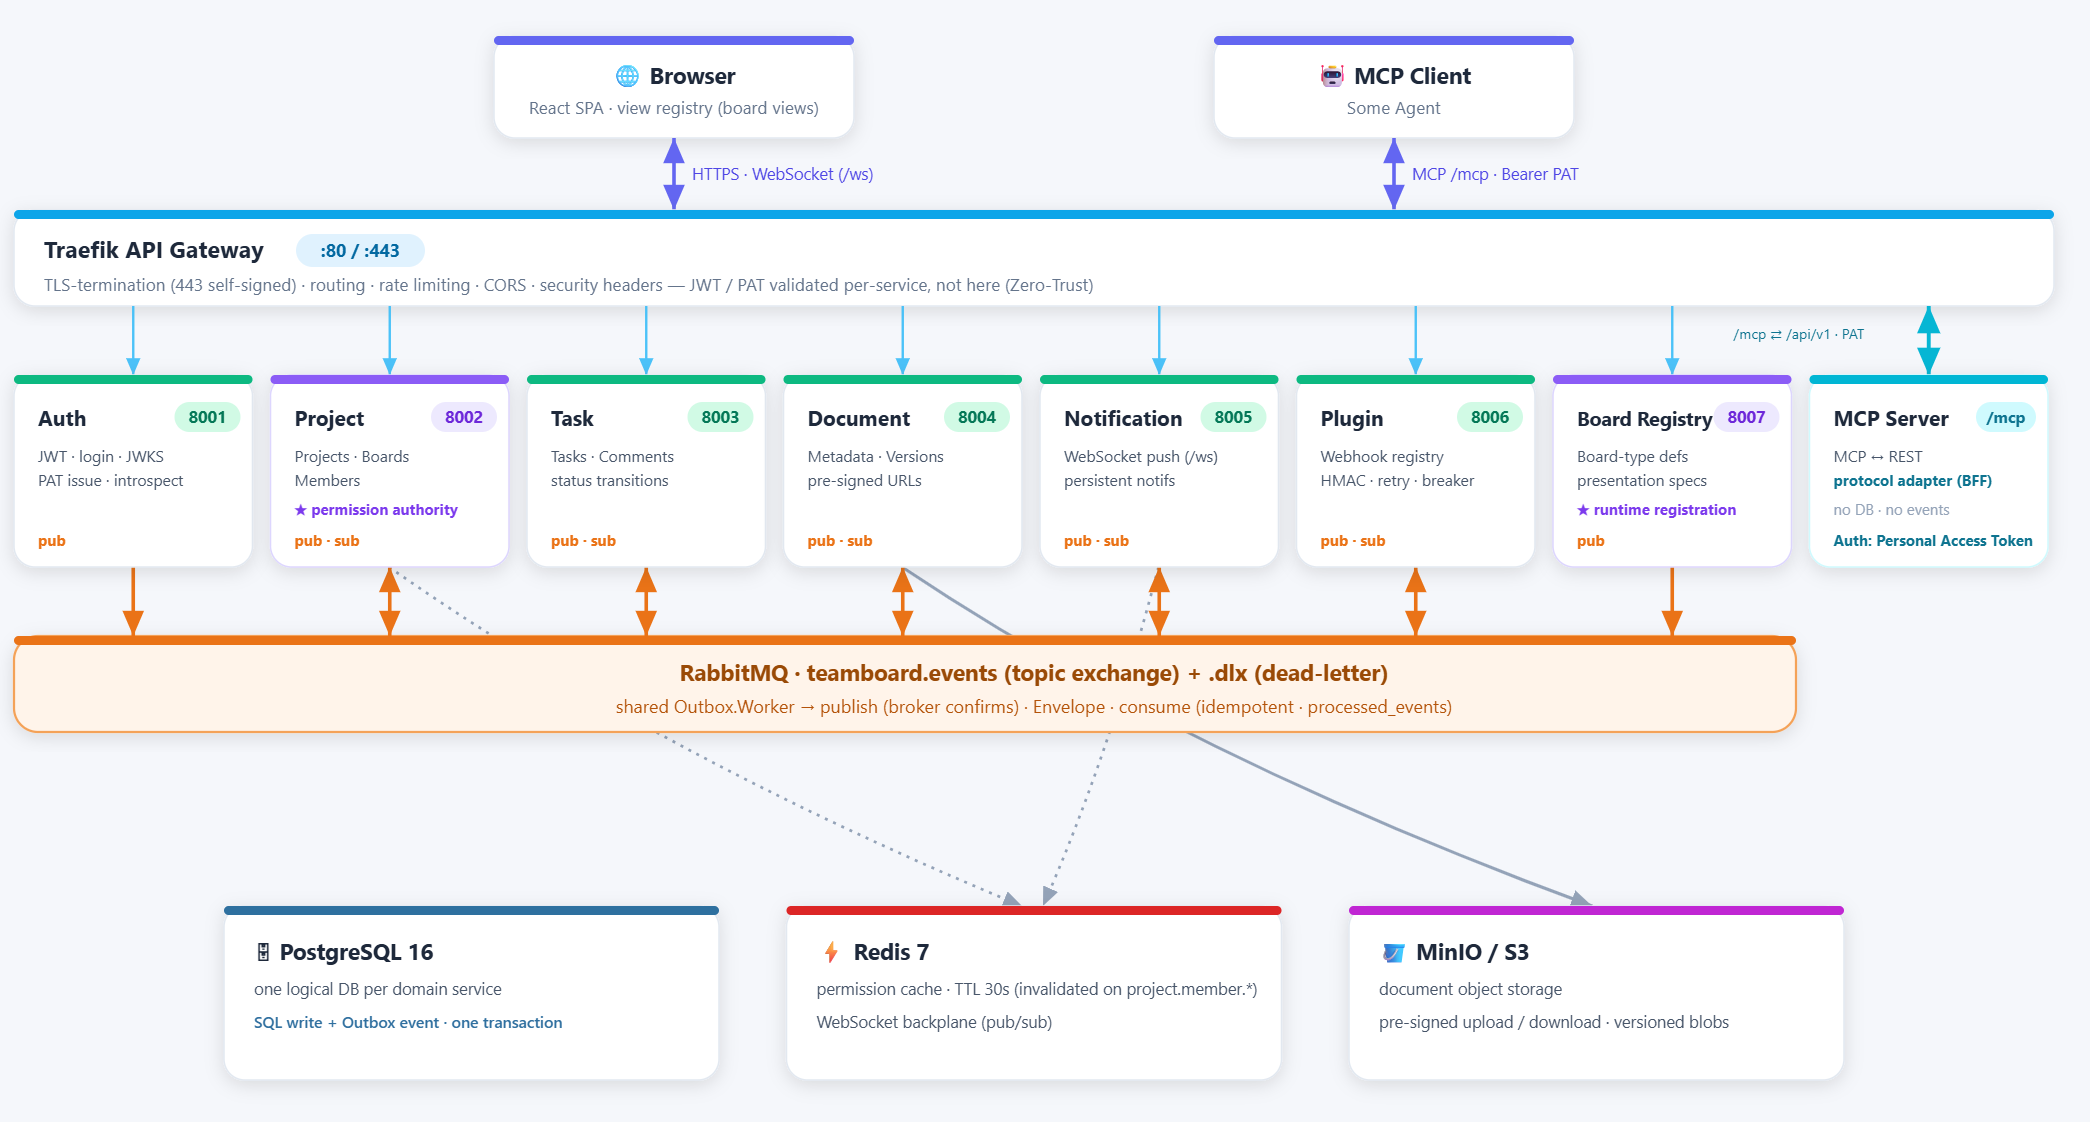
\includegraphics[width=\linewidth]{resources/plots/architecture.png}
  \caption{Gesamtarchitektur von TeamBoard mit Clients, Gateway, Diensten, Event-Bus und Infrastruktur.}
  \label{fig:architektur-gesamt}
\end{figure}

Die Grafik gliedert das System in horizontale Schichten. Ganz oben stehen die Clients, das Web-Frontend und der MCP-Client. Darunter liegt das Traefik-Gateway als einziger Eintrittspunkt, das Token bewusst nicht selbst prüft, sondern die Prüfung jedem Dienst überlässt. Es folgt die Reihe der fachlichen Dienste mit ihren Ports, ergänzt um den MCP-Server am rechten Rand. Darunter zieht sich der RabbitMQ-Event-Bus als gemeinsame Leitung durch das System. Am unteren Rand steht die Infrastruktur aus PostgreSQL, Redis und dem Objektspeicher. Die blauen Pfeile zeigen den Anfragefluss durch das Gateway, die orangen Pfeile das Veröffentlichen und Konsumieren von Ereignissen, die gestrichelten Linien die Anbindung an Cache und Objektspeicher. Die Grafik entstammt der Quelle im Repository unter \path{docs/architecture.svg}.

Drei Merkmale prägen das Bild. Erstens ist das Gateway der einzige Eintrittspunkt, prüft aber selbst keine Token. Zweitens laufen fachliche Ereignisse über den Topic-Exchange, sodass kein Sender seine Empfänger kennt. Drittens hält jeder Dienst seine eigenen Daten, und nur der Notification-Service hält bewusst Zustand in Form offener WebSocket-Verbindungen.

\section{Die einzelnen Komponenten}
\label{sec:komponenten}

Dieser Abschnitt stellt die Komponenten vor. Die fachlich einfacheren Dienste werden knapp beschrieben, die Board Registry und der Plugin-Service sowie der MCP-Server ausführlicher, da ihre Entwurfsentscheidungen für die Erweiterbarkeit des Systems zentral sind.

\subsection{Auth-Service}
\label{sub:auth}

Der Auth-Service verantwortet Identität und Authentifizierung. Er übernimmt Registrierung, Login, Token-Refresh und den Passwort-Reset und stellt signierte JWT aus. Über einen JWKS-Endpunkt veröffentlicht er den öffentlichen Schlüssel, mit dem alle anderen Dienste die Token prüfen. Projektbezogene Rollen gehören ausdrücklich nicht in diesen Dienst. Zusätzlich verwaltet der Auth-Service langlebige Personal Access Tokens für externe Clients und löst sie auf Anfrage anderer Dienste auf.

\subsection{Project-Service}
\label{sub:project}

Der Project-Service verwaltet Projekte, Boards und Mitgliedschaften und ist die autoritative Quelle für Berechtigungen. Er entscheidet über Rollen und deren Rechte und beantwortet die Berechtigungsanfragen der übrigen Dienste. Beim Anlegen eines Boards löst er den gewählten Board-Typ zur Laufzeit über die Board Registry auf und validiert die Board-Konfiguration gegen das vom Typ gelieferte Schema. Die Board-Instanzen bleiben in seiner Hoheit, während die Typ-Definitionen in der Registry liegen.

\subsection{Task-Service}
\label{sub:task}

Der Task-Service verwaltet Aufgaben innerhalb eines Boards mit Statusübergängen, Zuweisungen, Fälligkeiten, Kommentaren und Anhang-Referenzen. Er führt einen Audit-Trail über Änderungen. Den fachlichen Status einer Spalte leitet er nicht mehr aus dem Spaltennamen ab, sondern übernimmt ihn aus den expliziten Status-Angaben, die über Ereignisse aus dem Board-Kontext eintreffen. Vor schreibenden Operationen prüft er die Berechtigung beim Project-Service.

\subsection{Document-Service}
\label{sub:document}

Der Document-Service verwaltet Dokumente als Metadaten mit Verweis auf einen Objektspeicher und unterstützt Versionierung. Die eigentlichen Dateien fließen über vorsignierte URLs direkt zwischen Client und Objektspeicher, sodass der Dienst selbst keine großen Datenmengen durchleiten muss. Jede neue Version erhält einen eigenen Objekt-Schlüssel, was den Zugriff auf frühere Stände erlaubt.

\subsection{Notification-Service}
\label{sub:notification}

Der Notification-Service liefert Echtzeit-Benachrichtigungen über WebSockets und speichert persistente Benachrichtigungen. Er ist die einzige bewusst zustandsbehaftete Komponente, da er offene Verbindungen hält. Um dennoch mehrere Instanzen betreiben zu können, dient Redis als Backplane. Ein Ereignis erreicht eine Instanz und wird über Redis an alle Instanzen verteilt, die jeweils ihre lokalen Verbindungen prüfen. Er konsumiert fachliche Ereignisse, filtert sie nach Berechtigungen und stellt sie an die betroffenen Benutzer zu.

\subsection{Plugin- und Webhook-Service}
\label{sub:plugin}

Der Plugin-Service ist der Erweiterungspunkt für ausgehende Integrationen. Er konsumiert fachliche Ereignisse vom Event-Bus, filtert sie je Integration, überführt sie in ein Zielformat und stellt sie an externe Systeme zu. Der Kern der Entwurfsentscheidung ist die Trennung der Zustellung von den fachlichen Diensten. Ein Domain-Service kennt seine Empfänger nicht und ruft externe Systeme nicht direkt auf. Stattdessen veröffentlicht er ein Ereignis, und der Plugin-Service übernimmt die Zustellung. Die Alternative, jeden Dienst selbst ausliefern zu lassen, hätte die Zustelllogik über das ganze System verteilt und jeden Dienst mit Empfängerwissen belastet.

Als erster und im aktuellen Umfang einziger Integrationstyp ist der Webhook umgesetzt. Die Zustellung ist als Pipeline mit mehreren Schutzmechanismen ausgelegt. Ausgehende Aufrufe werden mit einer HMAC-Signatur versehen, sodass der Empfänger die Echtheit prüfen kann. Fehlgeschlagene Zustellungen werden mit exponentiellem Backoff wiederholt, und dauerhaft nicht erreichbare Ziele werden über einen Circuit Breaker je Webhook abgeschaltet. Nicht zustellbare Nachrichten landen in einer Dead-Letter-Queue. Ein Audit-Log hält jeden Zustellversuch fest. Weitere Kanäle wie E-Mail oder Chat-Dienste ließen sich als zusätzliche Plugins im selben Dienst ergänzen, ohne die Domain-Services zu berühren.

Da die Ziel-URL eines Webhooks vom Benutzer stammt, ist der ausgehende Aufruf eine Angriffsfläche für Server-Side Request Forgery. Ohne Schutz ließe sich ein interner Dienst als Ziel eintragen und über den Plugin-Service ansprechen. Der Dienst begegnet dem auf mehreren Ebenen. Bei der Registrierung werden nur die Schemata \texttt{http} und \texttt{https} zugelassen, der Hostname wird aufgelöst, und jede private, Loopback-, Link-Local- oder Cloud-Metadata-Adresse wird abgewiesen. Zusätzlich gilt eine Whitelist erlaubter Ports. Da sich die aufgelöste Adresse zwischen Registrierung und Zustellung ändern kann, prüft ein eigener Dialer die Zieladresse unmittelbar vor jedem Verbindungsaufbau erneut und verhindert so DNS-Rebinding. Dieselbe Prüfung greift bei jedem Redirect, und die Größe der Antwort ist begrenzt.

\subsection{Board Registry}
\label{sub:boardregistry}

Die Board Registry ist die autoritative Quelle für Board-Typ-Definitionen und erlaubt die Registrierung neuer Board-Typen zur Laufzeit. Eine Typ-Definition enthält die Default-Spalten mit ihrem jeweiligen Status, eine Default-Konfiguration, ein JSON-Schema zur Validierung der Board-Konfiguration und eine deklarative Presentation-Spezifikation für die Darstellung.

Der Entwurf ist in ADR 0001 festgehalten und diskutiert vier Optionen. Die ursprüngliche Umsetzung registrierte Board-Typen zur Compile-Zeit als Go-Pakete im Project-Service. Sie war typsicher, verlangte aber für jeden neuen Typ einen erneuten Build und ein Deployment und schloss externe Entwickler aus. Eine daten- und konfigurationsgetriebene Variante direkt im Project-Service hätte den zusätzlichen Dienst vermieden, aber die Registry-Verantwortung mit dem Eigentümer der Board-Instanzen vermischt. Code-Plugins über Go-Plugins oder WebAssembly hätten die höchste Mächtigkeit geboten, waren aber wegen Build-Fragilität auf der Windows-Entwicklungsumgebung und wegen des Sicherheits- und Betriebsrisikos nicht tragbar. Gewählt wurde ein eigener Registry-Dienst. Der Project-Service bezieht die Definitionen zur Laufzeit über eine interne Schnittstelle mit Cache und Service-Token und invalidiert den Cache über Ereignisse. Der Preis ist ein zusätzlicher, gecachter Synchron-Aufruf im Board-Erstellungspfad.

Die Darstellung der Boards ist in ADR 0002 gelöst. Da das Frontend eine kompilierte Single-Page-Anwendung ist, kann ein zur Laufzeit registrierter Typ keinen beliebigen Anzeigecode mitbringen. Die Presentation-Spezifikation beschreibt die Darstellung daher deklarativ. Eine View-Registry im Frontend wählt anhand eines Feldes den passenden eingebauten Renderer und fällt bei Unbekanntem auf die Spaltendarstellung zurück. Dieses eine Feld ist der einzige Erweiterungspunkt. Ein künftiger Renderer für entfernt geladene Views ist in ADR 0003 als Richtungsentscheidung beschrieben, aber bewusst noch nicht umgesetzt.

\subsection{MCP-Server}
\label{sub:mcp}

Der MCP-Server bindet Sprachmodell-Clients wie Claude an das System an. Er ist kein Domain-Service, sondern ein Protokoll-Adapter nach dem Muster eines Backend-for-Frontend. Er übersetzt eingehende Tool-Aufrufe des Model-Context-Protocol in die internen REST-Verträge und besitzt daher keine eigene Datenbank, keine Ereignisse und keinen Zustand. Seine Werkzeuge decken denselben Umfang ab wie die Weboberfläche, von Projekten und Boards über Aufgaben und Kommentare bis zur Registrierung neuer Board-Typen. Die Aufrufe gehen dabei bewusst über das Gateway und nicht direkt an die Dienste, sodass dieselben Routing-, CORS- und Rate-Limit-Regeln greifen wie für jeden anderen Client. Der Nutzen dieses Zuschnitts liegt darin, dass ein neuer Client-Typ neben dem Web-Frontend angebunden wird, ohne dass ein Domain-Service den fremden Client oder sein Protokoll kennen muss. Die Dienste bleiben von der Anbindung unberührt.

Die Authentifizierung dieses Zugangs war die eigentliche Entwurfsfrage. Ein Sprachmodell-Client ist ein fremdes Programm, das dauerhaft im Namen eines Benutzers handelt. Der erste Weg dorthin waren Personal Access Tokens, die ein Benutzer in den Einstellungen erzeugt und im Client hinterlegt. Sie sind bewusst opake Zeichenketten und keine selbst-validierenden JWT, denn ein langlebiges JWT wäre bis zu seinem Ablauf nicht widerrufbar. Ein Präfix im Token erlaubt der geteilten Auth-Middleware, es ohne Parse-Versuch an die Introspektion des Auth-Service zu leiten. Deren Ergebnis wird kurz zwischengespeichert und über einen Circuit Breaker gegen einen Ausfall abgesichert. Damit folgt der Entwurf demselben Muster wie die bestehenden Refresh-Tokens. Kurzlebige selbst-validierende Token tragen die Sitzung, während langlebige Zugänge über ein widerrufbares Token mit Serverzustand laufen.

Dieser Weg genügte jedoch nur für Clients, bei denen sich ein statisches Token hinterlegen lässt, und blieb damit praktisch auf die Kommandozeilenvariante beschränkt. Die Desktop-Anwendung von Claude bindet einen MCP-Server stattdessen als sogenannten Connector ein. Der Benutzer trägt dort lediglich eine URL ein, woraufhin die Anwendung den Zugang selbst über OAuth aushandelt. Ein Feld für ein vorab erzeugtes Token sieht dieser Ablauf nicht vor, sodass sich der Dienst über diesen Weg gar nicht erst anbinden ließ. Damit der Zugang nicht auf die Kommandozeile beschränkt bleibt, wurde der Auth-Service deshalb zusätzlich zum OAuth-2.1-Autorisierungsserver ausgebaut. Er veröffentlicht die Metadaten für Autorisierungsserver und geschützte Ressource und stellt Token über den Authorization-Code-Fluss mit PKCE aus. Da der Connector-Ablauf auch keine Gelegenheit bietet, eine Client-Kennung zu hinterlegen, registrieren sich die Clients selbst beim Autorisierungsserver. Der MCP-Server tritt als Ressourcenserver auf und beantwortet einen unauthentifizierten Aufruf mit einer Challenge, die beim Client die Metadaten-Suche und damit den gesamten Ablauf auslöst. Für den Benutzer reduziert sich die Einrichtung darauf, eine URL einzutragen und sich im Browser mit seinem gewohnten Konto anzumelden.

Bemerkenswert ist an dieser Stelle, wie wenig sich dadurch am übrigen System ändert. Das ausgestellte Zugriffstoken ist ein gewöhnliches TeamBoard-JWT und durchläuft Gateway, Dienste und Middleware unverändert. Die kurzlebigen Autorisierungscodes und die registrierten Clients liegen in Redis und erforderten keine Schemaänderung. Kein Domain-Service kennt OAuth. Die gesamte Erweiterung bleibt auf den Auth-Service und den Protokoll-Adapter beschränkt, was den Zuschnitt beider Komponenten im Nachhinein bestätigt.

\subsection{API-Gateway und Frontend}
\label{sub:gateway-frontend}

Das API-Gateway auf Basis von Traefik ist der einzige Eintrittspunkt. Es übernimmt Routing, Rate-Limiting, CORS und Sicherheits-Header und terminiert im Betrieb TLS. Geschäftslogik und Token-Prüfung liegen bewusst nicht im Gateway.

Das Frontend ist eine mit React und TypeScript umgesetzte Single-Page-Anwendung. Der Serverzustand wird über eine Query-Bibliothek zwischengespeichert, sodass die Oberfläche ohne manuelles Nachladen konsistent bleibt. Die View-Registry hält drei eingebaute Renderer bereit, eine Spaltendarstellung für Kanban, eine Kalender- und eine Timeline-Ansicht. Der Renderer wird anhand des Feldes \texttt{presentation.view} des Board-Typs gewählt, unbekannte Werte fallen auf die Spaltendarstellung zurück.

Ein Schwerpunkt des Frontends liegt auf der unmittelbaren Reaktion in gemeinsam genutzten Projekten. Bearbeiten mehrere Personen dasselbe Board, wird eine Änderung ohne Neuladen bei allen Beteiligten sichtbar. Diese Eigenschaft wird durch den ereignisgetriebenen Kern aus \vref{sec:zusammenspiel} getragen und reicht über den Notification-Service bis in die Oberfläche. Das Frontend hält je geöffnetem Board eine WebSocket-Verbindung, abonniert dessen Kanal und invalidiert bei einem eingehenden Aufgaben-Ereignis gezielt den lokalen Cache, worauf die betroffene Ansicht neu geladen wird.

\section{Zusammenspiel der Komponenten}
\label{sec:zusammenspiel}

Das Zusammenspiel folgt zwei Mustern. Ereignisse entkoppeln die Dienste, und wenige synchrone Aufrufe halten den Kern konsistent, wo eine sofortige verbindliche Antwort nötig ist.

Ein Beispiel für den asynchronen Weg ist das Verschieben einer Aufgabe. Der Task-Service veröffentlicht ein Ereignis über den Statuswechsel. Der Notification-Service konsumiert es und stellt eine Aktualisierung über WebSocket an die verbundenen Clients zu, sodass ein zweiter Browser die Änderung ohne Neuladen sieht. Der Plugin-Service kann dasselbe Ereignis konsumieren und einen signierten Webhook nach außen auslösen. Keiner der Empfänger kennt den anderen oder den Absender. Ein zusätzlicher Empfänger kostet nur einen weiteren Konsumenten und keine Änderung am Sender.

Ein Beispiel für den synchronen Weg ist das Anlegen eines Boards. Der Project-Service holt die Typ-Definition aus der Board Registry, da er sie unmittelbar zur Validierung braucht. Anschließend veröffentlicht er ein Ereignis über das angelegte Board, das die Spalten samt ihrem Status an den Task-Service trägt. Damit nutzt der Task-Service den fachlichen Status direkt, statt ihn aus Spaltennamen zu erraten.

Die Verlässlichkeit dieses Zusammenspiels beruht auf zwei Mechanismen. Das Outbox-Pattern stellt sicher, dass ein Ereignis genau dann existiert, wenn die zugehörige Datenänderung committet wurde. Idempotente Konsumenten stellen sicher, dass ein mehrfach zugestelltes Ereignis keinen Schaden anrichtet, indem sie verarbeitete Ereignis-Kennungen festhalten.

\vref{fig:ablauf-event} zeigt den beschriebenen asynchronen Ablauf als Sequenz. Der Task-Service legt das Ereignis über die Outbox auf den Event-Bus. Von dort konsumieren der Notification-Service und der Plugin-Service unabhängig voneinander. Der Notification-Service pusht die Aktualisierung an den Client, der Plugin-Service stellt einen signierten Webhook nach außen zu. Der Task-Service kennt keinen der beiden Empfänger.

\begin{figure}[ht]
  \centering
  \resizebox{\linewidth}{!}{%
  \begin{tikzpicture}[
      font=\small,
      head/.style={draw, rounded corners, fill=codeblue!10, align=center, minimum height=8mm, inner sep=3pt},
      msg/.style={-{Latex[length=2.2mm]}, thick},
      lifeline/.style={dashed, codegray},
    ]
    % Koepfe und Lebenslinien
    \foreach \x/\name in {0/Client, 2.7/Task-Service, 5.4/RabbitMQ, 8.1/Notification, 10.8/Plugin, 13.5/{Externes System}} {
      \node[head] at (\x,0) {\name};
      \draw[lifeline] (\x,-0.55) -- (\x,-6);
    }
    % Nachrichten
    \draw[msg] (2.7,-1.3) -- node[above, font=\scriptsize] {task.status.changed (Outbox)} (5.4,-1.3);
    \draw[msg] (5.4,-2.3) -- node[above, font=\scriptsize] {consume} (8.1,-2.3);
    \draw[msg] (8.1,-3.1) -- node[above, font=\scriptsize] {WebSocket-Push} (0,-3.1);
    \draw[msg] (5.4,-4.1) -- node[above, font=\scriptsize] {consume} (10.8,-4.1);
    \draw[msg] (10.8,-5.0) -- node[above, font=\scriptsize] {signierter Webhook} (13.5,-5.0);
  \end{tikzpicture}%
  }
  \caption{Sequenz eines Ereignisflusses beim Verschieben einer Aufgabe. Notification- und Plugin-Service konsumieren dasselbe Ereignis, ohne voneinander zu wissen.}
  \label{fig:ablauf-event}
\end{figure}

\section{Verweise auf das Repository}
\label{sec:repository-verweise}

Die ausführlichen Entwurfsunterlagen liegen im Repository. Der vorliegende Bericht fasst die zentralen Entscheidungen zusammen und verweist für die Details auf die folgenden Artefakte.

\begin{table}[ht]
  \centering
  \caption{Wichtige Entwurfsartefakte im Repository}
  \label{tab:repo-artefakte}
  \begin{tabularx}{\linewidth}{@{}lX@{}}
    \toprule
    \textbf{Artefakt} & \textbf{Inhalt} \\
    \midrule
    \path{docs/ARCHITECTURE.md}               & Master-Referenz, Prinzipien, Service-Katalog, Event-Schema \\
    \path{docs/architecture-diagram.md}       & Quelle des Architekturdiagramms \\
    \path{docs/decisions/0001-...}            & ADR zur Laufzeit-Erweiterbarkeit der Board-Typen \\
    \path{docs/decisions/0002-...}            & ADR zur Erweiterbarkeit der Board-Darstellung \\
    \path{docs/decisions/0003-...}            & ADR zu entfernt geladenen Board-Views (Vorschlag) \\
    \path{docs/services/*.md}                  & Detail-Design je Dienst mit Datenmodell und Schnittstellen \\
    \path{docs/specifications/deployment.md}   & Deployment- und CI/CD-Beschreibung \\
    \bottomrule
  \end{tabularx}
\end{table}

\chapter{Realisierung und Implementierung}
\label{chap:realisierung}

\section{Gewählter Software-Stack}
\label{sec:software-stack}

\section{Vorgehen bei der Programmerstellung}
\label{sec:vorgehen}

\section{Einsatz von KI bei der Programmerstellung}
\label{sec:ki-programmerstellung}

\section{Herausforderungen bei der Realisierung}
\label{sec:herausforderungen}

\chapter{Deployment und Evaluation}
\label{chap:deployment}

\section{Voraussetzungen und Start des Systems}
\label{sec:start}

\section{Vorstellung des laufenden Systems}
\label{sec:laufendes-system}

\section{Realisierter Funktionsumfang}
\label{sec:funktionsumfang}

\chapter{Fazit und Ausblick}
\label{chap:fazit}

\section{Zusammenfassende Bewertung}
\label{sec:bewertung}

Die Aufgabenstellung verlangte kein möglichst umfangreiches Produkt, sondern eine tragfähige und skalierbare Architektur. Gemessen an diesem Maßstab wurde das Ziel erreicht, denn das TeamBoard ist ein lauffähiges Microservice-System aus sieben Diensten und einem Protokoll-Adapter, das lokal mit einem Kommando startet und über eine Push-Pipeline in die Cloud ausrollt. Der Fokus lag hierbei vor allem auf den gewählten Architekturen und nicht auf der Implementierung möglicher Features, weswegen die Funktionalität  bewusst schlank blieb. Der in \vref{sec:funktionsumfang} zusammengefasste Funktionsumfang belegt beides, den umgesetzten Kern und die bewusst offen gehaltenen Lücken für zukünftige Weiterentwicklungen.

Die drei Leitfragen aus \vref{sec:kontext} bilden den roten Faden dieser Bewertung. An ihnen lässt sich am ehesten ablesen, wie gut die gewählte Architektur ihren eigenen Anspruch einlöst.

\paragraph{Verteilung von Echtzeit-Ereignissen.} Die erste Frage ist am deutlichsten beantwortet. Der ereignisgetriebene Kern aus \vref{sec:zusammenspiel} übernimmt die Verteilung von Echtzeit-Ereignissen von Anfang bis Ende. Ein fachliches Ereignis wird über die Outbox verlässlich auf den RabbitMQ-Topic-Exchange gelegt, von mehreren Diensten unabhängig konsumiert und über den Notification-Service bis in die offene WebSocket-Verbindung des Clients zugestellt. Dass ein zweites Browser-Fenster eine verschobene Aufgabe ohne Neuladen sieht, ist dabei kein Sonderweg der Oberfläche, sondern die sichtbare Wirkung dieses Kerns. Entscheidend ist dabei die Entkopplung, so dass ein zusätzlicher Empfänger, wie z.B. ein Webhook über den Plugin-Service, nur einen weiteren Konsumenten kostet und keine Änderung am Sender bedarf. Der Preis dieses Weges ist die Eventual Consistency nach außen, die allerdings über idempotente Verarbeitung und eine Dead-Letter-Queue beherrschbar bleibt.

\paragraph{Unabhängige Skalierbarkeit.} Die zweite Frage fällt zwiespältiger aus und verdient die ehrlichste Antwort. Die unabhängige Skalierbarkeit ist im Entwurf konsequent angelegt, im laufenden Betrieb aber nicht ausgespielt. Alle Dienste außer dem Notification-Service sind zustandslos, besitzen ihre eigene Datenbank und werden allein über Umgebungsvariablen konfiguriert, sodass sich jeder Dienst grundsätzlich einzeln vervielfachen ließe. Der bewusst gewählte Betrieb auf einer einzigen EC2-Instanz aus \vref{sec:betriebsmodell} macht von dieser Eigenschaft jedoch keinen Gebrauch. Diese Entscheidung war unter den Rahmenbedingungen des Projekts richtig, denn sie hält lokale und produktive Umgebung identisch und die Kosten minimal. Sie hat aber den erkennbaren Preis eines Single Point of Failure und eines Betriebs, in dem von der geforderten Skalierbarkeit nichts zu sehen ist. Der Zuschnitt der Dienste sorgt allerdings dafür, dass der Weg zu echter Skalierung ein Ausbau bestehender Kanten bleibt und keine Neuentwicklung erfordert. Insofern ist die Frage im Entwurf beantwortet, im Betrieb jedoch nur vorbereitet.

\paragraph{Konsistenter Datenzugriff.} Die dritte Frage beantwortet die Architektur über eine bewusste Zweiteilung. Wo eine sofortige verbindliche Antwort nötig ist, ermöglicht ein schmaler synchroner Kern die Konsistenz. Der Project-Service ist die alleinige Autorität für Berechtigungen, und der Board-Typ wird beim Anlegen eines Boards synchron aus der Board Registry aufgelöst. Überall sonst wird Konsistenz über Ereignisse hergestellt und ist damit letztlich konsistent statt sofort. Die Verlässlichkeit dieses Ansatzes ruht auf zwei Mechanismen: Zum Einen stellt das Outbox-Pattern sicher, dass ein Ereignis genau dann existiert, wenn die zugehörige Datenänderung committet wurde, und zum Anderen sorgen idempotente Konsumenten dafür, dass eine mehrfache Übermittlung keinen Schaden anrichtet. Die getrennten Datenbanken je Dienst ermöglichen diese Autonomie damit, dass fachübergreifende Sichten nicht per SQL-Join, sondern über Ereignisse und Schnittstellen zusammengeführt werden. Für den gewählten Zuschnitt ist dieser Tausch angemessen.

Über die drei Leitfragen hinaus hat sich der Grundzug des Entwurfs, Erweiterungen auf klar benannte Punkte zu beschränken, im Verlauf des Projekts mehrfach bestätigt. Am deutlichsten zeigt sich das an der nachträglichen Anbindung von Sprachmodell-Clients aus \vref{sub:mcp}. Der Ausbau des Auth-Service zum OAuth-2.1-Autorisierungsserver blieb auf den Auth-Service und den Protokoll-Adapter beschränkt, ohne dass ein Domain-Service davon berührt wurde oder ein Schema sich änderte. Ebenso ist die Laufzeit-Registrierung neuer Board-Typen aus \vref{sub:boardregistry} über die Nutzung des Notebooks aus \vref{sec:laufendes-system} im laufenden System nachvollziehbar. Solche Belege sind aus unserer Sicht der eigentliche Ertrag des Projekts, da sie den Anspruch der Architektur an konkreten Erweiterungen einlösen.

Zugleich bleiben die in \vref{sec:funktionsumfang} benannten Lücken bestehen und werden hier nicht schöngeredet. Zwei offene Punkte betreffen die Autorisierung, nämlich die noch nicht auf eine Administrationsrolle eingeschränkten Schreibrouten der Board Registry und die fehlende synchrone Mitgliedschaftsprüfung beim Abonnieren eines Board-Kanals. Beide sind bekannt, dokumentiert und im vorliegenden Stand bewusst nicht umgesetzt. Dass diese Lücken offen genannt werden, ist die Konsequenz aus einer während des Projekts wiederholt beobachteten Neigung der Dokumentation, dem Code vorauszulaufen, wie in \vref{sec:ki-programmerstellung} beschrieben.

\section{Ausblick}
\label{sec:ausblick}

Aus der Bewertung ergeben sich mehrere Richtungen für die Weiterentwicklung, die sich in drei Gruppen ordnen lassen. Sie bauen durchweg auf dem bestehenden Entwurf auf und verlangen keine grundlegende Neukonzeption.

Die erste und naheliegendste Gruppe schließt die bekannten Lücken und behebt bekannte Probleme. Die Schreibrouten der Board Registry wären auf eine Administrationsrolle einzuschränken, und der Notification-Service benötigt eine Zuordnung von Boards zu Projekten, um die Mitgliedschaft beim Abonnieren eines Kanals synchron prüfen zu können. Diese Zuordnung ließe sich über die bereits vorhandenen Ereignisse des Project-Service aufbauen und fügt sich damit in den ereignisgetriebenen Kern ein. Hinzu käme der noch fehlende Test des Tracing-Exportpfads, der einen eigenen Test-Collector erfordert. Diese Arbeiten erhöhen den bestehenden Funktionsumfang nicht, sondern bringen den realisierten Stand auf das im Entwurf angelegte Sicherheitsniveau.

Die zweite Gruppe spielt die Skalierbarkeit aus, die bislang nur vorbereitet ist. Der in \vref{sec:betriebsmodell} skizzierte Weg führt in drei Schritten weiter, die den Anwendungscode unberührt lassen. Zuerst würden die zustandsbehafteten Container in verwaltete Dienste ausgelagert, also PostgreSQL nach RDS, Redis nach ElastiCache, RabbitMQ nach Amazon MQ und der Objektspeicher nach S3. Anschließend zögen die Dienste selbst auf eine Container-Plattform wie ECS oder Fargate um, wobei die vorhandenen Produktions-Images unverändert weiterlaufen. Zuletzt verteilte ein Load Balancer mehrere Instanzen je Dienst, was seinen Nutzen erst dann entfaltet, wenn einzelne Dienste tatsächlich unterschiedlich stark belastet werden. Erst dieser letzte Schritt macht aus der entworfenen Skalierbarkeit eine im Betrieb sichtbare Eigenschaft und schließt damit die zweite Leitfrage auch auf der Betriebsseite.

Die dritte Gruppe betrifft die fachliche und die konzeptionelle Erweiterung entlang der bereits angelegten Erweiterungspunkte. Der Plugin-Service ist als offener Punkt für ausgehende Integrationen entworfen, sodass sich neben dem umgesetzten Webhook weitere Kanäle wie E-Mail oder Chat-Dienste als zusätzliche Plugins ergänzen ließen, ohne die Domain-Services zu berühren. Ebenso sind eingehende Webhooks noch offen. Bei der Darstellung der Boards ist mit der Presentation-Spezifikation und dem einen Erweiterungsfeld \texttt{presentation.view} der Rahmen für entfernt geladene Views bereits gesetzt. Der in ADR 0003 als Richtungsentscheidung beschriebene Renderer für einen Wert \texttt{view:\,\enquote{remote}} würde diesen Rahmen ausfüllen und echte Micro-Frontends erlauben, ohne das zugrunde liegende Modell zu ändern. Dass eine solche Erweiterung ohne Eingriff in die bestehenden Dienste möglich ist, war das Ziel des Entwurfs und bleibt die aussagekräftigste Prüfung seiner Tragfähigkeit.

Insgesamt zeigt der Ausblick, dass die tragenden Entscheidungen dieses Projekts nicht auf den erreichten Stand begrenzt sind, sondern einen Weg für die Weiterentwicklung vorzeichnen. Der bewusste Verzicht auf funktionale Breite zugunsten einer sauber geschnittenen Architektur zahlt sich genau an dieser Stelle aus, denn jede der genannten Erweiterungen ist ein Ausbau des Bestehenden und erfordert keine einschneidenden Anpassungen.

\end{onehalfspace}

%%%%%%%%%%%%%%%%%%%%%%%%%%%%%%%%%%%%%%%%%%%%%%%%%%%%%%%%%%%%%%%%%%%

\printbibliography{} % create with BibTeX, gives "chapter without number" warning in log

% \appendix
% \include{stuff/anhang}

\end{document}
